%!TEX root = ../Demo.tex
\chapter{The IoC Container}
This chapter covers Spring’s Inversion of Control (IoC) container.

\section{Introduction to the Spring IoC Container and Beans}
This chapter covers the Spring Framework implementation of the Inversion of Control (IoC)
principle. IoC is also known as dependency injection (DI). It is a process whereby objects define
their dependencies (that is, the other objects they work with) only through constructor arguments,
arguments to a factory method, or properties that are set on the object instance after it is
constructed or returned from a factory method. The container then injects those dependencies
when it creates the bean. This process is fundamentally the inverse (hence the name, Inversion of
Control) of the bean itself controlling the instantiation or location of its dependencies by using
direct construction of classes or a mechanism such as the Service Locator pattern.

The org.springframework.beans and org.springframework.context packages are the basis for Spring
Framework’s IoC container. The BeanFactory interface provides an advanced configuration
mechanism capable of managing any type of object. ApplicationContext is a sub-interface of
BeanFactory. It adds:

\begin{itemize}
    \item Easier integration with Spring’s AOP features
    \item Message resource handling (for use in internationalization)
    \item Event publication
    \item Application-layer specific contexts such as the WebApplicationContext for use in web
    applications.
\end{itemize}

In short, the BeanFactory provides the configuration framework and basic functionality, and the
ApplicationContext adds more enterprise-specific functionality. The ApplicationContext is a
complete superset of the BeanFactory and is used exclusively in this chapter in descriptions of
Spring’s IoC container. For more information on using the BeanFactory instead of the
ApplicationContext, see The BeanFactory.

In Spring, the objects that form the backbone of your application and that are managed by the
Spring IoC container are called beans. A bean is an object that is instantiated, assembled, and
managed by a Spring IoC container. Otherwise, a bean is simply one of many objects in your
application. Beans, and the dependencies among them, are reflected in the configuration metadata
used by a container.

\section{Container Overview}
The org.springframework.context.ApplicationContext interface represents the Spring IoC container
and is responsible for instantiating, configuring, and assembling the beans. The container gets its
instructions on what objects to instantiate, configure, and assemble by reading configuration
metadata. The configuration metadata is represented in XML, Java annotations, or Java code. It lets
you express the objects that compose your application and the rich interdependencies between those objects.

Several implementations of the ApplicationContext interface are supplied with Spring. In standalone applications, it is common to create an instance of ClassPathXmlApplicationContext or
FileSystemXmlApplicationContext. While XML has been the traditional format for defining
configuration metadata, you can instruct the container to use Java annotations or code as the
metadata format by providing a small amount of XML configuration to declaratively enable support
for these additional metadata formats.

In most application scenarios, explicit user code is not required to instantiate one or more
instances of a Spring IoC container. For example, in a web application scenario, a simple eight (or
so) lines of boilerplate web descriptor XML in the web.xml file of the application typically suffices
(see Convenient ApplicationContext Instantiation for Web Applications). If you use the Spring Tools
for Eclipse (an Eclipse-powered development environment), you can easily create this boilerplate
configuration with a few mouse clicks or keystrokes.

The following diagram shows a high-level view of how Spring works. Your application classes are
combined with configuration metadata so that, after the ApplicationContext is created and
initialized, you have a fully configured and executable system or application.

\begin{figure}[ht]
    \centering
    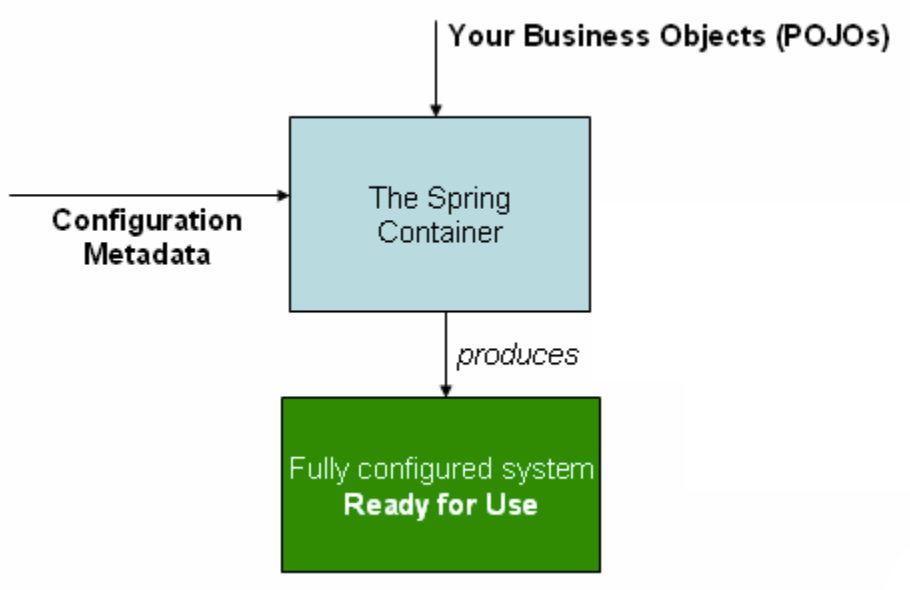
\includegraphics[width=0.6\linewidth]{./Figure/IMG_process.png}
    \caption{The Spring IoC container}\label{Fig:xd1}
  \end{figure}


\subsection{Configuration Metadata}
As the preceding diagram shows, the Spring IoC container consumes a form of configuration
metadata. This configuration metadata represents how you, as an application developer, tell the
Spring container to instantiate, configure, and assemble the objects in your application.

Configuration metadata is traditionally supplied in a simple and intuitive XML format, which is
what most of this chapter uses to convey key concepts and features of the Spring IoC container.

For information about using other forms of metadata with the Spring container, see:

\begin{itemize}
    \item Annotation-based configuration: Spring 2.5 introduced support for annotation-based
    configuration metadata.
    \item  Java-based configuration: Starting with Spring 3.0, many features provided by the Spring
    JavaConfig project became part of the core Spring Framework. Thus, you can define beans
    external to your application classes by using Java rather than XML files. To use these new
    features, see the @Configuration, @Bean, @Import, and @DependsOn annotations.
\end{itemize}

Spring configuration consists of at least one and typically more than one bean definition that the
container must manage. XML-based configuration metadata configures these beans as <bean/>
elements inside a top-level <beans/> element. Java configuration typically uses @Bean-annotated
methods within a @Configuration class.

These bean definitions correspond to the actual objects that make up your application. Typically,
you define service layer objects, data access objects (DAOs), presentation objects such as Struts
Action instances, infrastructure objects such as Hibernate SessionFactories, JMS Queues, and so
forth. Typically, one does not configure fine-grained domain objects in the container, because it is
usually the responsibility of DAOs and business logic to create and load domain objects. However,
you can use Spring’s integration with AspectJ to configure objects that have been created outside
the control of an IoC container. See Using AspectJ to dependency-inject domain objects with Spring.

The following example shows the basic structure of XML-based configuration metadata:

\begin{figure}[ht]
    \centering
    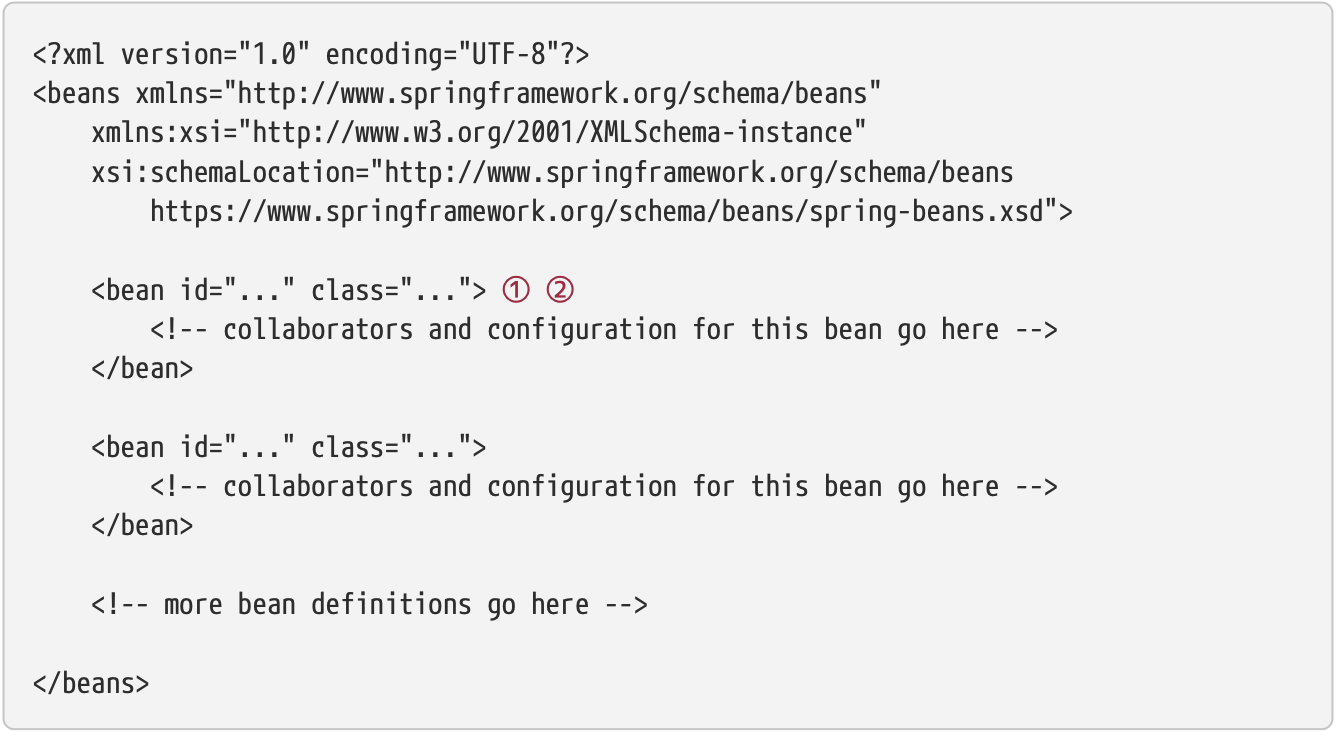
\includegraphics[width=1\linewidth]{./Figure/IMG_code_1.png}
  \end{figure}

  \begin{enumerate}
    \item The id attribute is a string that identifies the individual bean definition.
    \item The class attribute defines the type of the bean and uses the fully qualified classname.
\end{enumerate}

The value of the id attribute refers to collaborating objects. The XML for referring to collaborating
objects is not shown in this example. See Dependencies for more information.

\subsection{Instantiating a Container}
The location path or paths supplied to an ApplicationContext constructor are resource strings that
let the container load configuration metadata from a variety of external resources, such as the local
file system, the Java CLASSPATH, and so on.

\begin{figure}[ht]
    \centering
    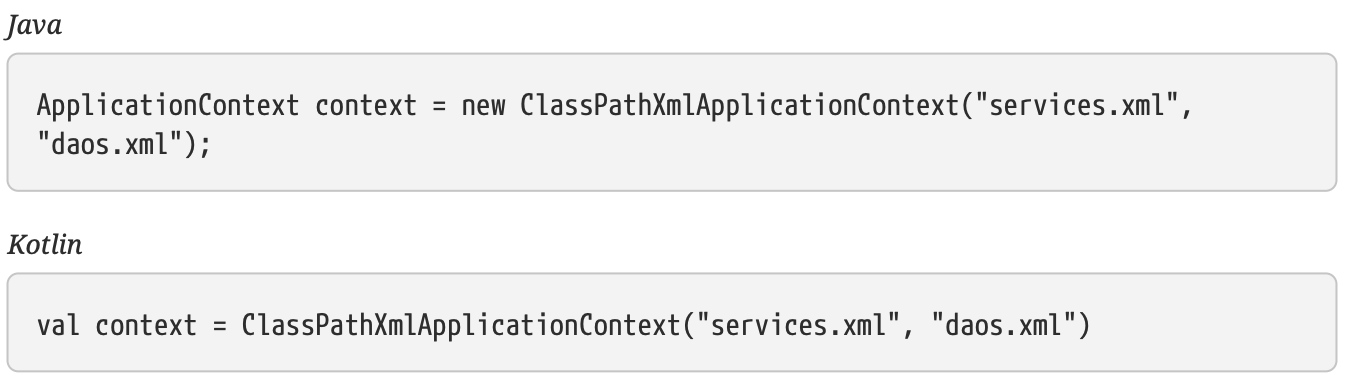
\includegraphics[width=1\linewidth]{./Figure/IMG_code_2.png}
  \end{figure}

The following example shows the service layer objects (services.xml) configuration file:

\begin{figure}[ht]
\centering
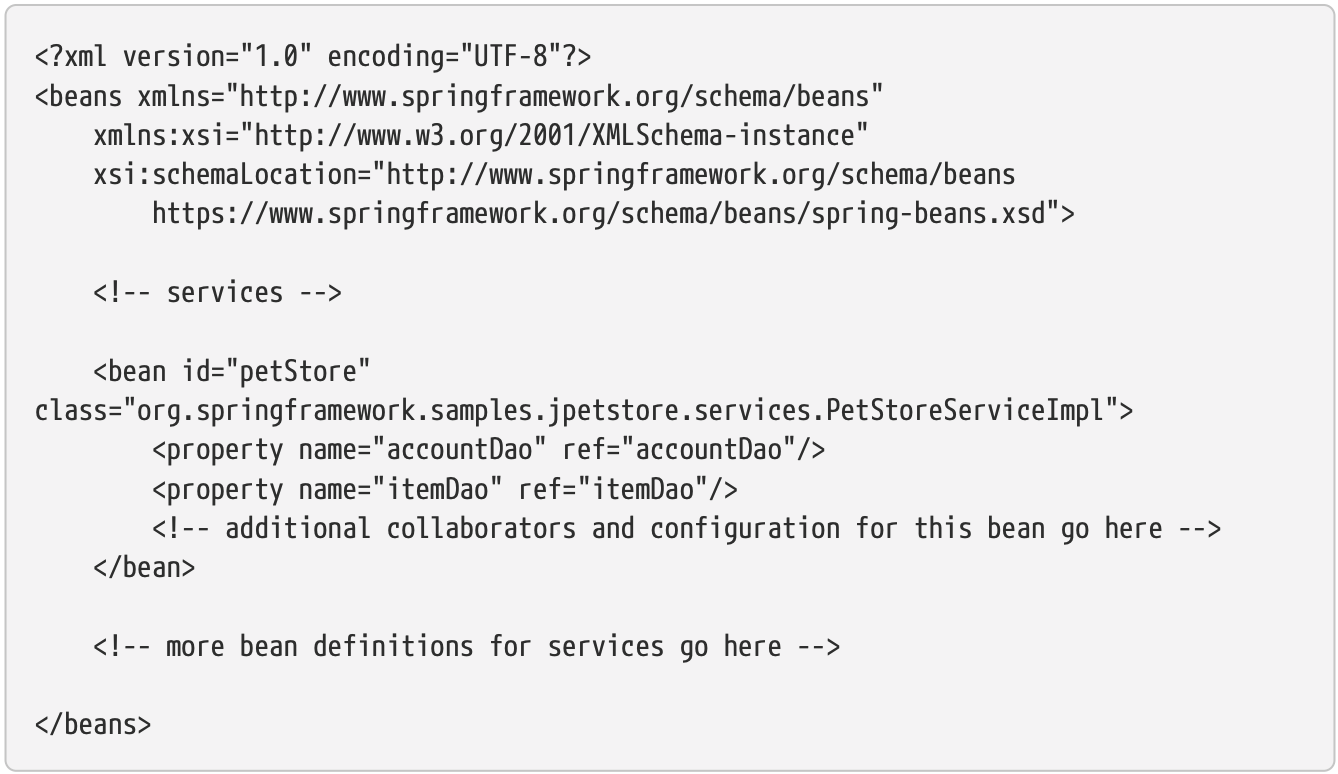
\includegraphics[width=1\linewidth]{./Figure/IMG_code_3.png}
\end{figure}

\newpage
The following example shows the data access objects daos.xml file:

\begin{figure}[ht]
\centering
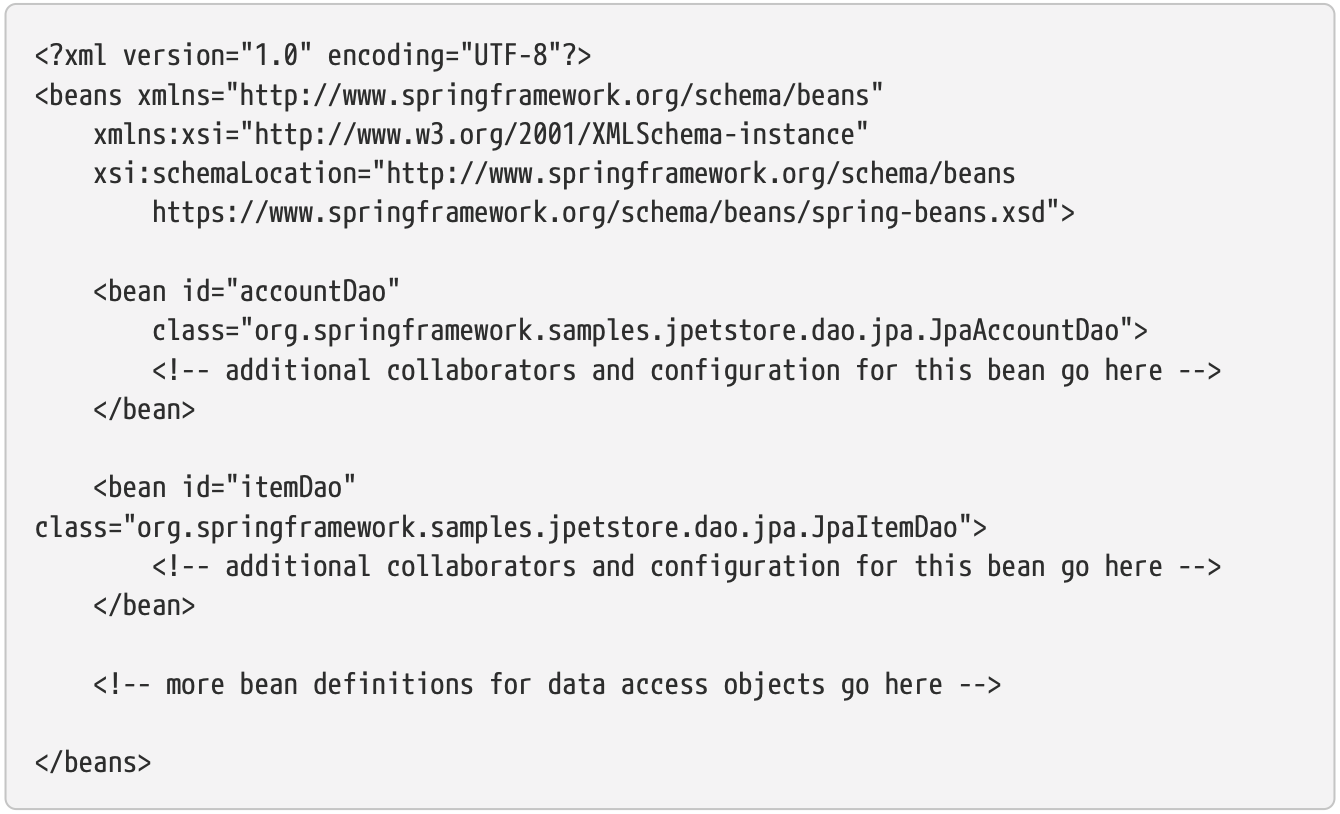
\includegraphics[width=1\linewidth]{./Figure/IMG_code_4.png}
\end{figure}

In the preceding example, the service layer consists of the PetStoreServiceImpl class and two data
access objects of the types JpaAccountDao and JpaItemDao (based on the JPA Object-Relational
Mapping standard). The property name element refers to the name of the JavaBean property, and the
ref element refers to the name of another bean definition. This linkage between id and ref
elements expresses the dependency between collaborating objects. For details of configuring an
object’s dependencies, see Dependencies.

\subsubsection{Composing XML-based Configuration Metadata}
It can be useful to have bean definitions span multiple XML files. Often, each individual XML
configuration file represents a logical layer or module in your architecture.

You can use the application context constructor to load bean definitions from all these XML
fragments. This constructor takes multiple Resource locations, as was shown in the previous section.
Alternatively, use one or more occurrences of the <import/> element to load bean definitions from
another file or files. The following example shows how to do so:

\newpage
\begin{figure}[ht]
\centering
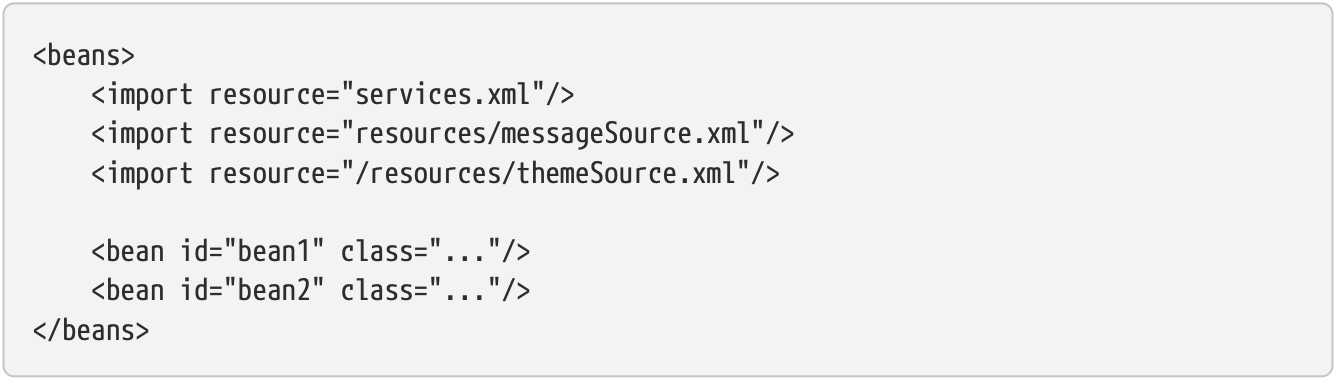
\includegraphics[width=1\linewidth]{./Figure/IMG_code_5.png}
\end{figure}

In the preceding example, external bean definitions are loaded from three files: services.xml,
messageSource.xml, and themeSource.xml. All location paths are relative to the definition file doing
the importing, so services.xml must be in the same directory or classpath location as the file doing
the importing, while messageSource.xml and themeSource.xml must be in a resources location below
the location of the importing file. As you can see, a leading slash is ignored. However, given that
these paths are relative, it is better form not to use the slash at all. The contents of the files being
imported, including the top level <beans/> element, must be valid XML bean definitions, according
to the Spring Schema.

The namespace itself provides the import directive feature. Further configuration features beyond
plain bean definitions are available in a selection of XML namespaces provided by Spring — for
example, the context and util namespaces.

\subsubsection{The Groovy Bean Definition DSL}

As a further example for externalized configuration metadata, bean definitions can also be
expressed in Spring’s Groovy Bean Definition DSL, as known from the Grails framework. Typically,
such configuration live in a ".groovy" file with the structure shown in the following example:

\newpage
\begin{figure}[ht]
\centering
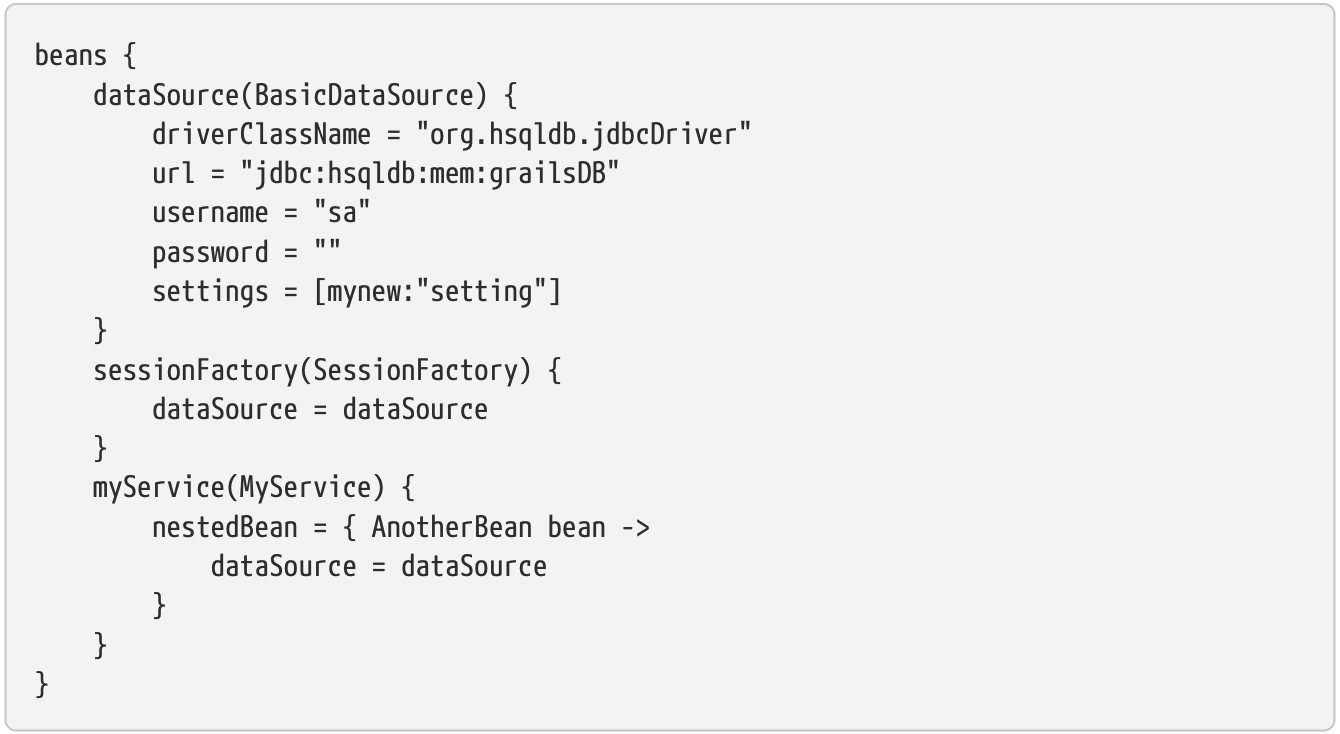
\includegraphics[width=1\linewidth]{./Figure/IMG_code_6.png}
\end{figure}

This configuration style is largely equivalent to XML bean definitions and even supports Spring’s
XML configuration namespaces. It also allows for importing XML bean definition files through an
importBeans directive.

\subsection{Using the Container}

The ApplicationContext is the interface for an advanced factory capable of maintaining a registry of
different beans and their dependencies. By using the method T getBean(String name, Class<T>
requiredType), you can retrieve instances of your beans.


The ApplicationContext lets you read bean definitions and access them, as the following example
shows:

\begin{figure}[ht]
    \centering
    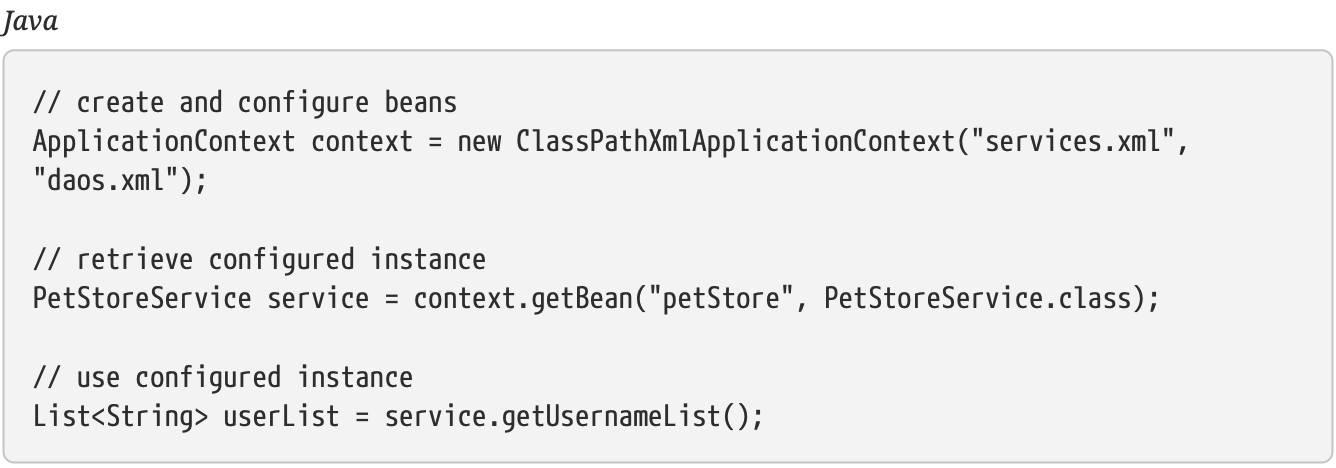
\includegraphics[width=1\linewidth]{./Figure/IMG_code_7.png}
\end{figure}

\newpage
\begin{figure}[ht]
    \centering
    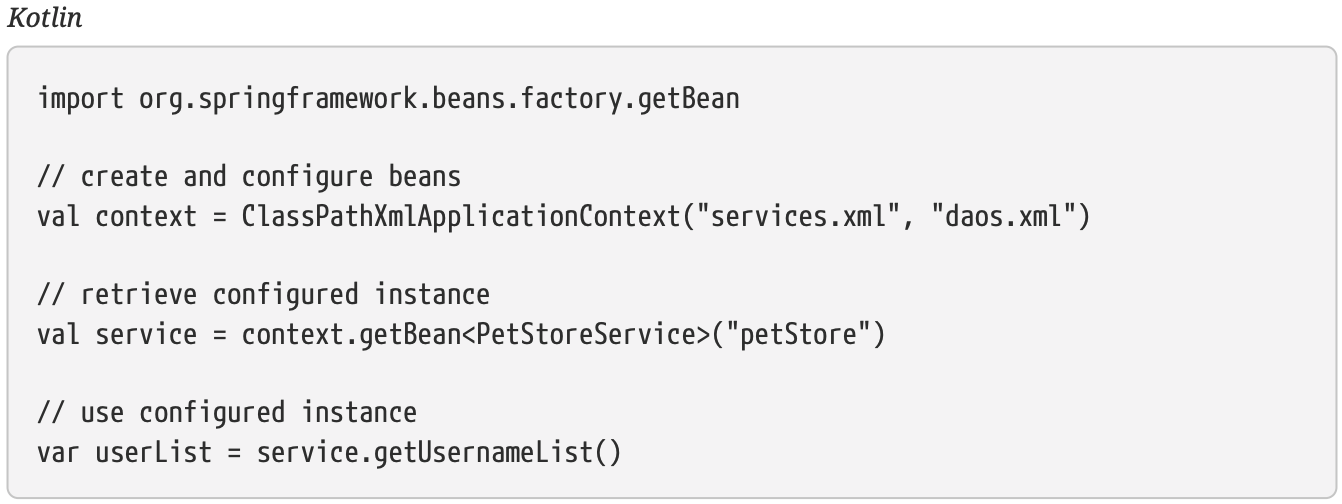
\includegraphics[width=1\linewidth]{./Figure/IMG_code_8.png}
\end{figure}

With Groovy configuration, bootstrapping looks very similar. It has a different context
implementation class which is Groovy-aware (but also understands XML bean definitions). The
following example shows Groovy configuration:

\begin{figure}[ht]
    \centering
    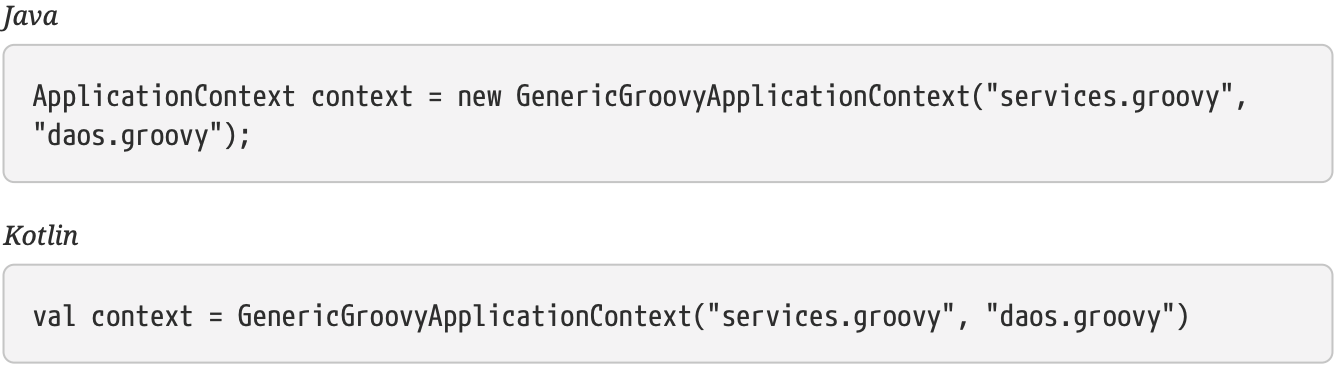
\includegraphics[width=1\linewidth]{./Figure/IMG_code_9.png}
\end{figure}

The most flexible variant is GenericApplicationContext in combination with reader delegates — for
example, with XmlBeanDefinitionReader for XML files, as the following example shows:

\begin{figure}[ht]
    \centering
    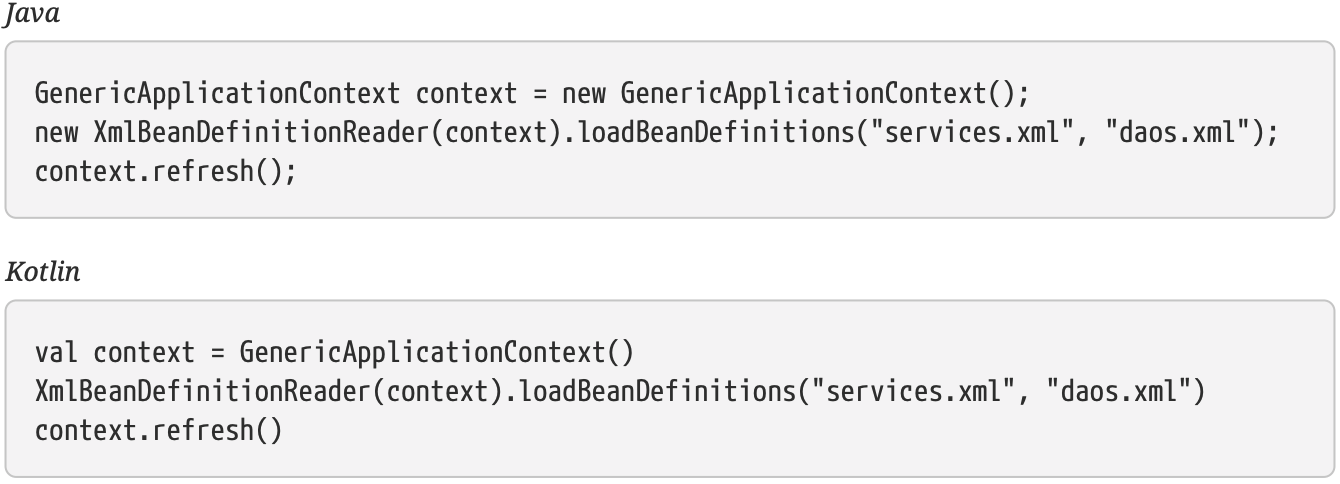
\includegraphics[width=1\linewidth]{./Figure/IMG_code_10.png}
\end{figure}

\newpage
You can also use the GroovyBeanDefinitionReader for Groovy files, as the following example shows:

\begin{figure}[ht]
    \centering
    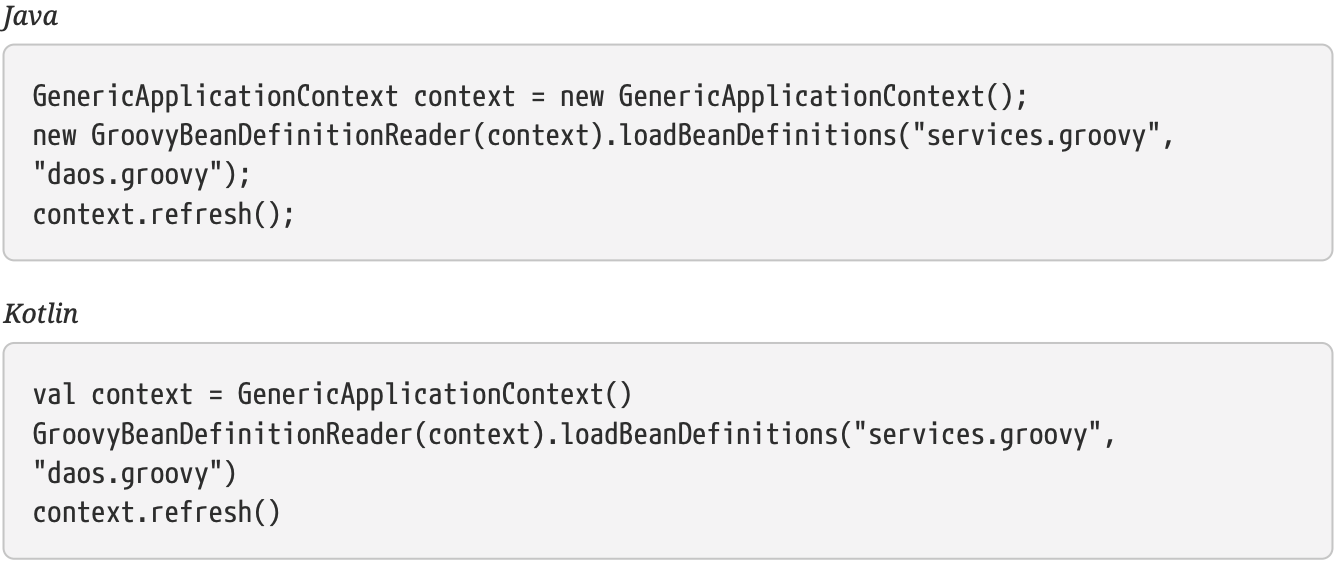
\includegraphics[width=1\linewidth]{./Figure/IMG_code_11.png}
\end{figure}

You can mix and match such reader delegates on the same ApplicationContext, reading bean
definitions from diverse configuration sources.

You can then use getBean to retrieve instances of your beans. The ApplicationContext interface has a
few other methods for retrieving beans, but, ideally, your application code should never use them.
Indeed, your application code should have no calls to the getBean() method at all and thus have no
dependency on Spring APIs at all. For example, Spring’s integration with web frameworks provides
dependency injection for various web framework components such as controllers and JSF-managed
beans, letting you declare a dependency on a specific bean through metadata (such as an
autowiring annotation).

\section{Bean Overview}
A Spring IoC container manages one or more beans. These beans are created with the configuration
metadata that you supply to the container (for example, in the form of XML <bean/> definitions).
Within the container itself, these bean definitions are represented as BeanDefinition objects, which
contain (among other information) the following metadata:

\begin{itemize}
    \item A package-qualified class name: typically, the actual implementation class of the bean being
    defined.
    \item Bean behavioral configuration elements, which state how the bean should behave in the
    container (scope, lifecycle callbacks, and so forth).
    \item References to other beans that are needed for the bean to do its work. These references are also
    called collaborators or dependencies.
    \item Other configuration settings to set in the newly created object — for example, the size limit of
    the pool or the number of connections to use in a bean that manages a connection pool.
\end{itemize}

This metadata translates to a set of properties that make up each bean definition. The following
table describes these properties:


\begin{figure}[ht]
    \centering
    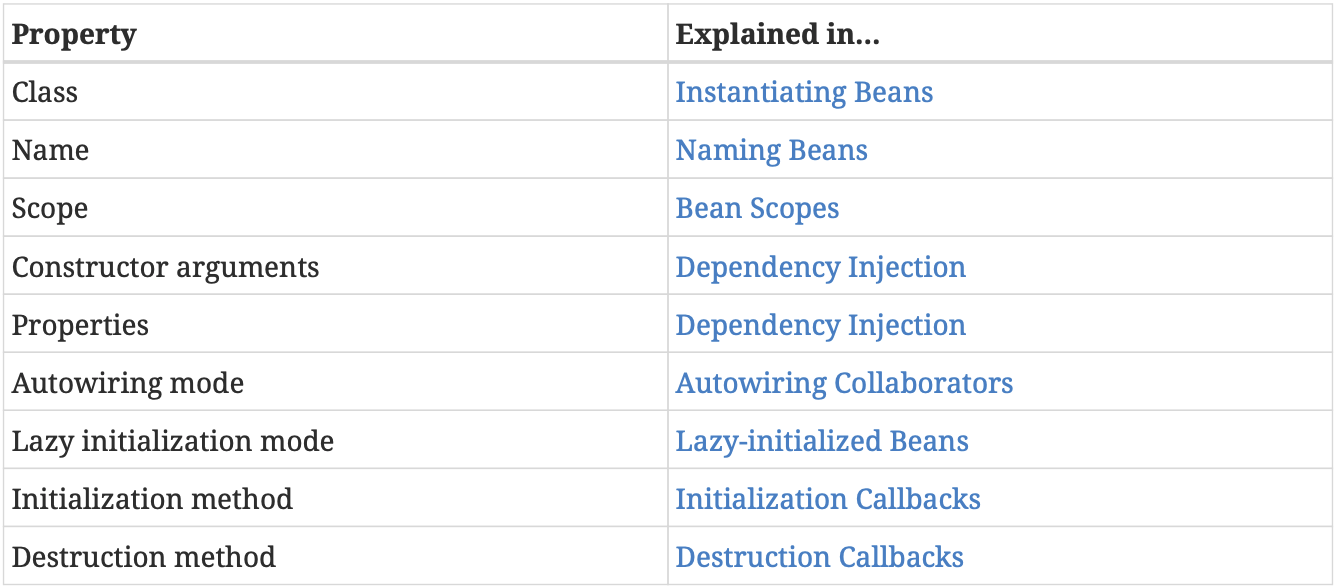
\includegraphics[width=1\linewidth]{./Figure/IMG_bean_def.png}
\end{figure}

In addition to bean definitions that contain information on how to create a specific bean, the
ApplicationContext implementations also permit the registration of existing objects that are created
outside the container (by users). This is done by accessing the ApplicationContext’s BeanFactory
through the getBeanFactory() method, which returns the BeanFactory DefaultListableBeanFactory
implementation. DefaultListableBeanFactory supports this registration through the
registerSingleton(..) and registerBeanDefinition(..) methods. However, typical applications
work solely with beans defined through regular bean definition metadata.


\subsection{Naming Beans}

Every bean has one or more identifiers. These identifiers must be unique within the container that
hosts the bean. A bean usually has only one identifier. However, if it requires more than one, the
extra ones can be considered aliases.

In XML-based configuration metadata, you use the id attribute, the name attribute, or both to specify
the bean identifiers. The id attribute lets you specify exactly one id. Conventionally, these names
are alphanumeric ('myBean', 'someService', etc.), but they can contain special characters as well. If
you want to introduce other aliases for the bean, you can also specify them in the name attribute,
separated by a comma (,), semicolon (;), or white space. As a historical note, in versions prior to
Spring 3.1, the id attribute was defined as an xsd:ID type, which constrained possible characters. As
of 3.1, it is defined as an xsd:string type. Note that bean id uniqueness is still enforced by the
container, though no longer by XML parsers.

You are not required to supply a name or an id for a bean. If you do not supply a name or id explicitly,
the container generates a unique name for that bean. However, if you want to refer to that bean by
name, through the use of the ref element or a Service Locator style lookup, you must provide a
name. Motivations for not supplying a name are related to using inner beans and autowiring
collaborators.

\subsubsection{Aliasing a Bean outside the Bean Definition}
In a bean definition itself, you can supply more than one name for the bean, by using a
combination of up to one name specified by the id attribute and any number of other names in the
name attribute. These names can be equivalent aliases to the same bean and are useful for some
situations, such as letting each component in an application refer to a common dependency by
using a bean name that is specific to that component itself.

Specifying all aliases where the bean is actually defined is not always adequate, however. It is
sometimes desirable to introduce an alias for a bean that is defined elsewhere. This is commonly
the case in large systems where configuration is split amongst each subsystem, with each
subsystem having its own set of object definitions. In XML-based configuration metadata, you can
use the <alias/> element to accomplish this. The following example shows how to do so:

\begin{figure}[ht]
    \centering
    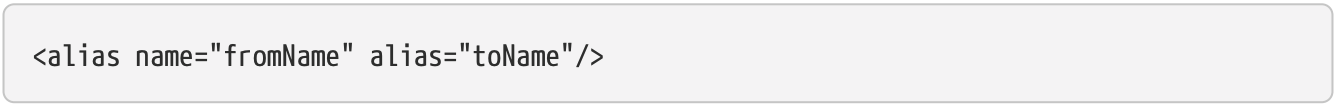
\includegraphics[width=1\linewidth]{./Figure/IMG_code_12.png}
\end{figure}

In this case, a bean (in the same container) named fromName may also, after the use of this alias
definition, be referred to as toName.

For example, the configuration metadata for subsystem A may refer to a DataSource by the name of
subsystemA-dataSource. The configuration metadata for subsystem B may refer to a DataSource by
the name of subsystemB-dataSource. When composing the main application that uses both these
subsystems, the main application refers to the DataSource by the name of myApp-dataSource. To have
all three names refer to the same object, you can add the following alias definitions to the
configuration metadata:

\begin{figure}[ht]
    \centering
    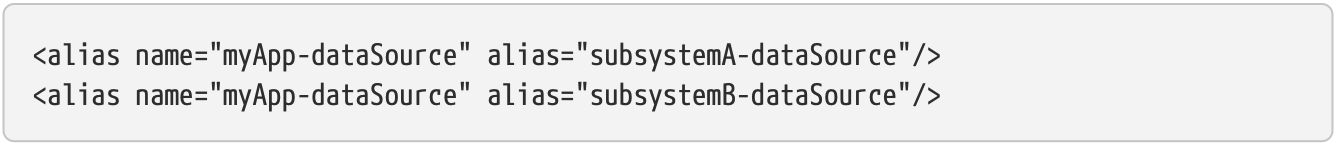
\includegraphics[width=1\linewidth]{./Figure/IMG_code_13.png}
\end{figure}

\section{Instantiating Beans}
A bean definition is essentially a recipe for creating one or more objects. The container looks at the
recipe for a named bean when asked and uses the configuration metadata encapsulated by that
bean definition to create (or acquire) an actual object.

If you use XML-based configuration metadata, you specify the type (or class) of object that is to be
instantiated in the class attribute of the <bean/> element. This class attribute (which, internally, is a
Class property on a BeanDefinition instance) is usually mandatory. (For exceptions, see
Instantiation by Using an Instance Factory Method and Bean Definition Inheritance.) You can use
the Class property in one of two ways:


\begin{itemize}
    \item Typically, to specify the bean class to be constructed in the case where the container itself
    directly creates the bean by calling its constructor reflectively, somewhat equivalent to Java
    code with the new operator.
    \item To specify the actual class containing the static factory method that is invoked to create the
    object, in the less common case where the container invokes a static factory method on a class
    to create the bean. The object type returned from the invocation of the static factory method
    may be the same class or another class entirely.
\end{itemize}

\subsubsection{Instantiation with a Constructor}
When you create a bean by the constructor approach, all normal classes are usable by and
compatible with Spring. That is, the class being developed does not need to implement any specific
interfaces or to be coded in a specific fashion. Simply specifying the bean class should suffice.
However, depending on what type of IoC you use for that specific bean, you may need a default
(empty) constructor.

The Spring IoC container can manage virtually any class you want it to manage. It is not limited to
managing true JavaBeans. Most Spring users prefer actual JavaBeans with only a default (noargument) constructor and appropriate setters and getters modeled after the properties in the
container. You can also have more exotic non-bean-style classes in your container. If, for example,
you need to use a legacy connection pool that absolutely does not adhere to the JavaBean
specification, Spring can manage it as well.

With XML-based configuration metadata you can specify your bean class as follows:

\begin{figure}[ht]
    \centering
    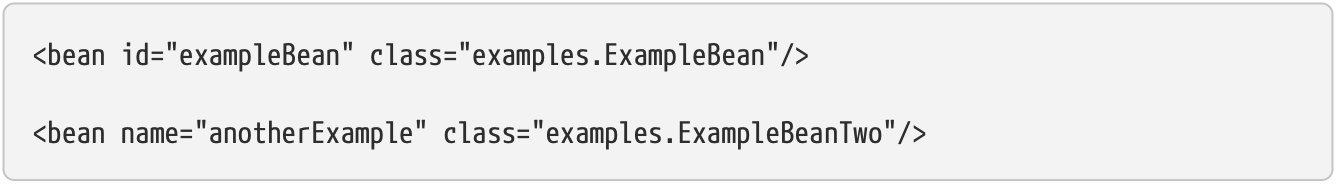
\includegraphics[width=1\linewidth]{./Figure/IMG_code_14.png}
\end{figure}

For details about the mechanism for supplying arguments to the constructor (if required) and
setting object instance properties after the object is constructed, see Injecting Dependencies.


\subsubsection{Instantiation with a Static Factory Method}
When defining a bean that you create with a static factory method, use the class attribute to specify
the class that contains the static factory method and an attribute named factory-method to specify
the name of the factory method itself. You should be able to call this method (with optional
arguments, as described later) and return a live object, which subsequently is treated as if it had
been created through a constructor. One use for such a bean definition is to call static factories in
legacy code.

The following bean definition specifies that the bean be created by calling a factory method. The
definition does not specify the type (class) of the returned object, only the class containing the
factory method. In this example, the createInstance() method must be a static method. The
following example shows how to specify a factory method:

\begin{figure}[ht]
    \centering
    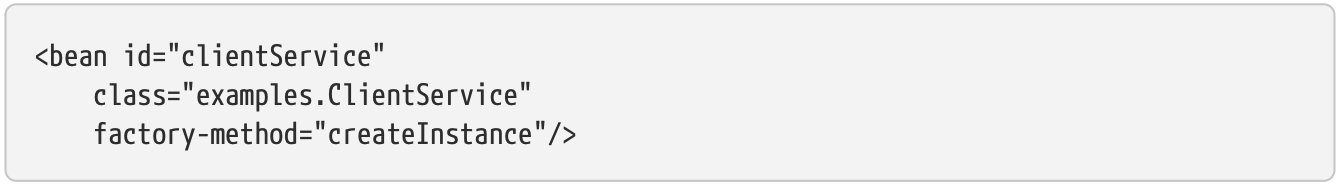
\includegraphics[width=1\linewidth]{./Figure/IMG_code_15.png}
\end{figure}

The following example shows a class that would work with the preceding bean definition:

\begin{figure}[ht]
    \centering
    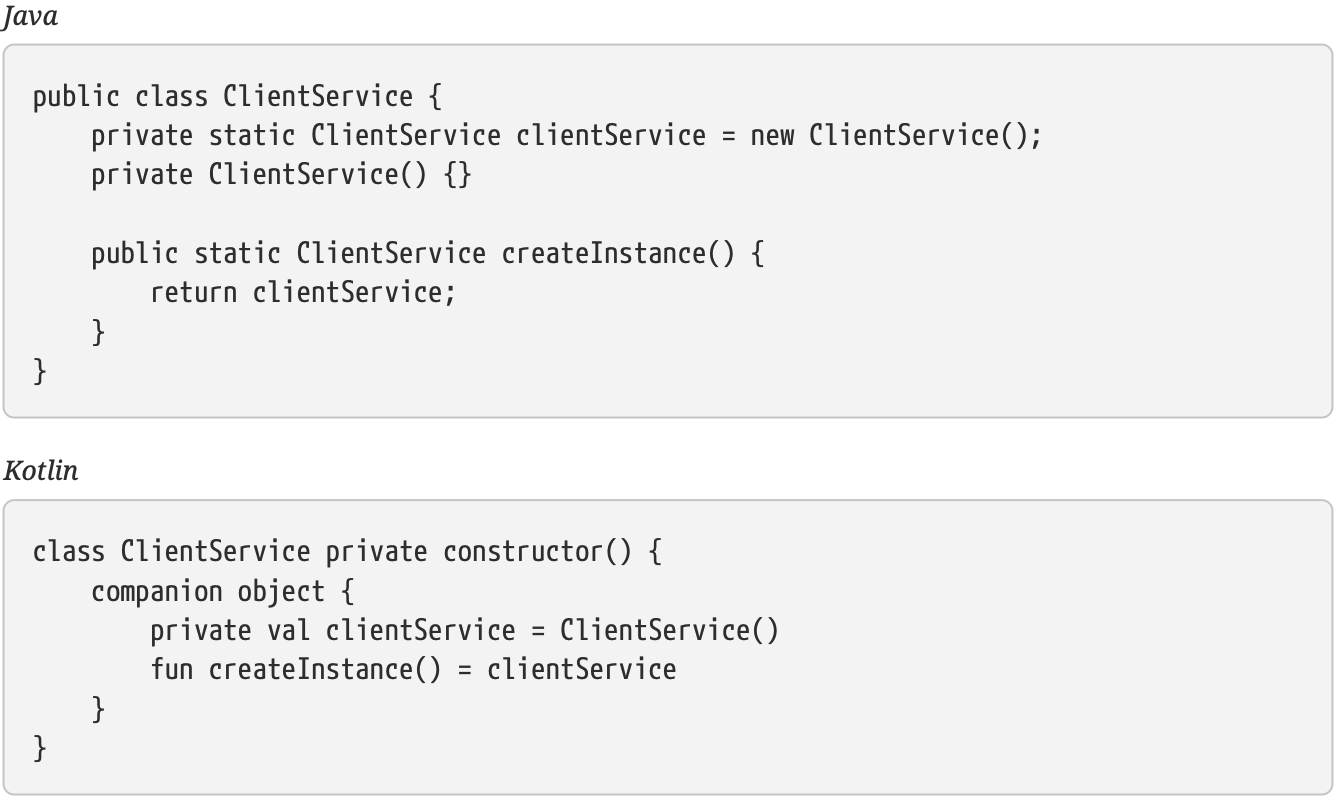
\includegraphics[width=1\linewidth]{./Figure/IMG_code_16.png}
\end{figure}

For details about the mechanism for supplying (optional) arguments to the factory method and
setting object instance properties after the object is returned from the factory, see Dependencies
and Configuration in Detail.

\subsubsection{Instantiation by Using an Instance Factory Method}
Similar to instantiation through a static factory method, instantiation with an instance factory
method invokes a non-static method of an existing bean from the container to create a new bean.
To use this mechanism, leave the class attribute empty and, in the factory-bean attribute, specify
the name of a bean in the current (or parent or ancestor) container that contains the instance
method that is to be invoked to create the object. Set the name of the factory method itself with the
factory-method attribute. The following example shows how to configure such a bean:

\begin{figure}[ht]
    \centering
    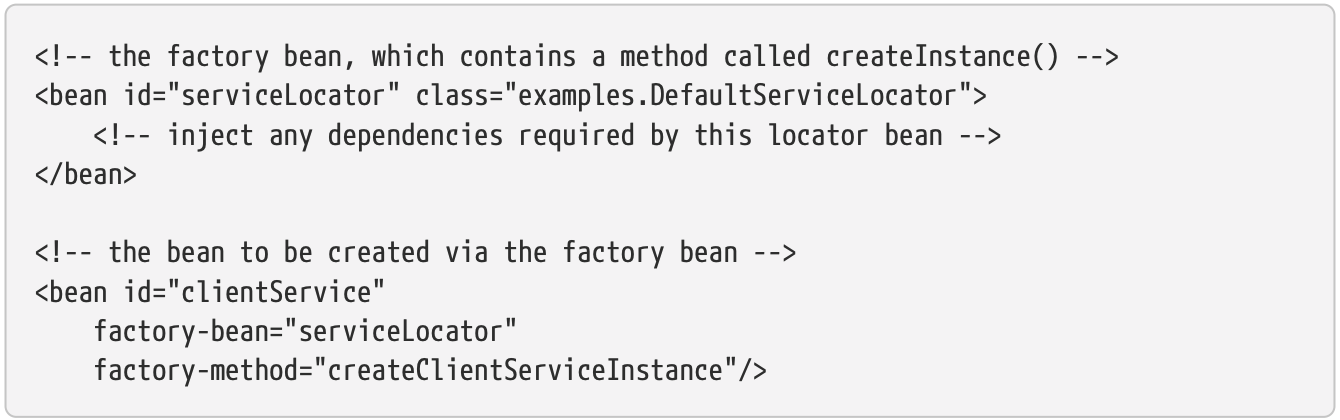
\includegraphics[width=1\linewidth]{./Figure/IMG_code_17.png}
\end{figure}

The following example shows the corresponding class:

\begin{figure}[ht]
    \centering
    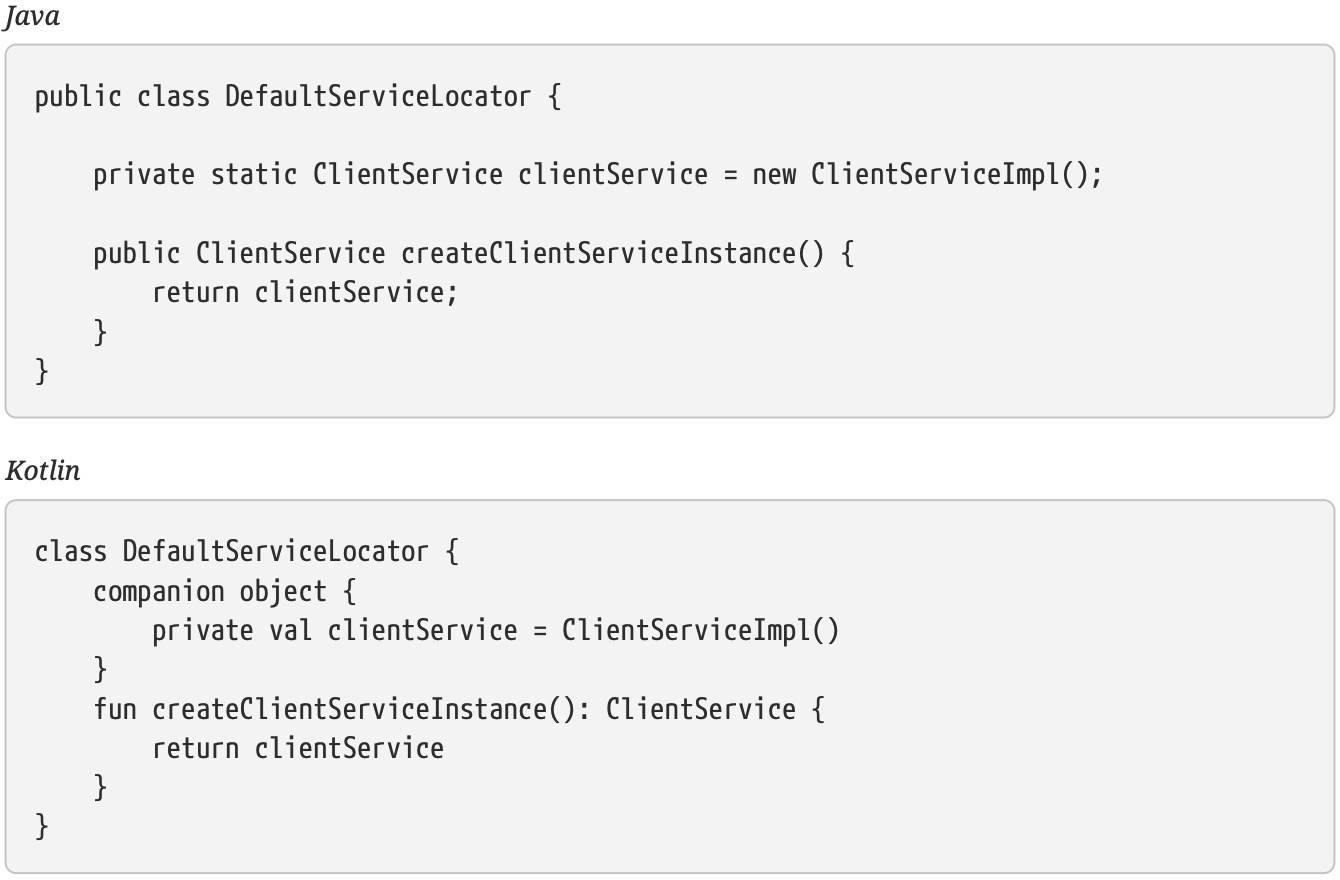
\includegraphics[width=1\linewidth]{./Figure/IMG_code_18.png}
\end{figure}

\newpage
One factory class can also hold more than one factory method, as the following example shows:

\begin{figure}[ht]
    \centering
    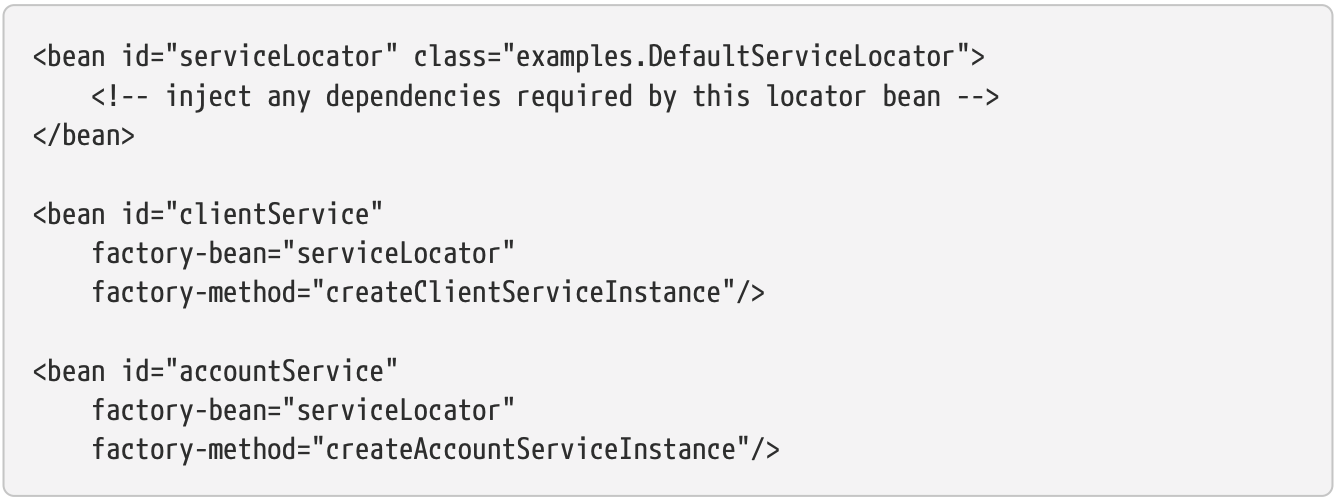
\includegraphics[width=1\linewidth]{./Figure/IMG_code_19.png}
\end{figure}

\newpage
The following example shows the corresponding class:

\begin{figure}[ht]
    \centering
    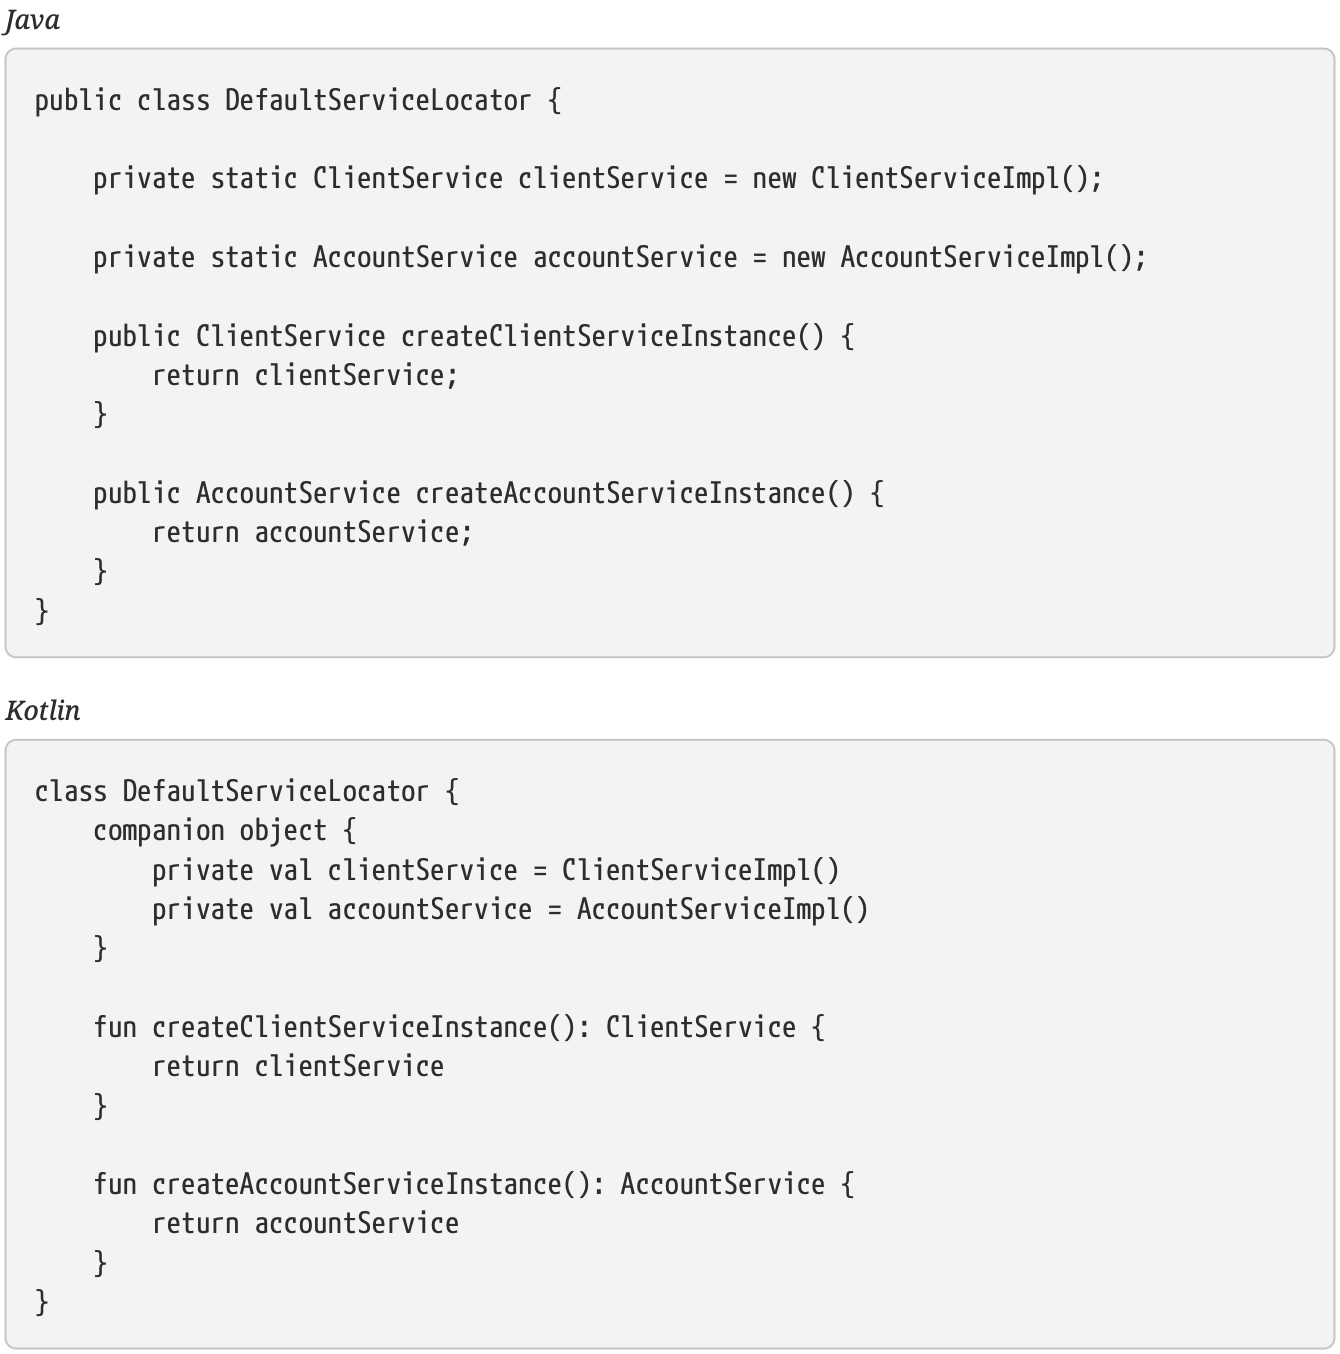
\includegraphics[width=1\linewidth]{./Figure/IMG_code_20.png}
\end{figure}

This approach shows that the factory bean itself can be managed and configured through
dependency injection (DI). See \textbf{Dependencies and Configuration in Detail}.

\subsubsection{Determining a Bean’s Runtime Type}
The runtime type of a specific bean is non-trivial to determine. A specified class in the bean
metadata definition is just an initial class reference, potentially combined with a declared factory
method or being a FactoryBean class which may lead to a different runtime type of the bean, or not
being set at all in case of an instance-level factory method (which is resolved via the specified
factory-bean name instead). Additionally, AOP proxying may wrap a bean instance with an
interface-based proxy with limited exposure of the target bean’s actual type (just its implemented
interfaces).

The recommended way to find out about the actual runtime type of a particular bean is a
BeanFactory.getType call for the specified bean name. This takes all of the above cases into account
and returns the type of object that a BeanFactory.getBean call is going to return for the same bean
name.

\section{Dependencies}
A typical enterprise application does not consist of a single object (or bean in the Spring parlance).
Even the simplest application has a few objects that work together to present what the end-user
sees as a coherent application. This next section explains how you go from defining a number of
bean definitions that stand alone to a fully realized application where objects collaborate to achieve
a goal.

\subsection{Dependency Injection}
Dependency injection (DI) is a process whereby objects define their dependencies (that is, the other
objects with which they work) only through constructor arguments, arguments to a factory method,
or properties that are set on the object instance after it is constructed or returned from a factory
method. The container then injects those dependencies when it creates the bean. This process is
fundamentally the inverse (hence the name, Inversion of Control) of the bean itself controlling the
instantiation or location of its dependencies on its own by using direct construction of classes or the
Service Locator pattern.

Code is cleaner with the DI principle, and decoupling is more effective when objects are provided
with their dependencies. The object does not look up its dependencies and does not know the
location or class of the dependencies. As a result, your classes become easier to test, particularly
when the dependencies are on interfaces or abstract base classes, which allow for stub or mock
implementations to be used in unit tests.

DI exists in two major variants: Constructor-based dependency injection and Setter-based
dependency injection.

\subsubsection{Constructor-based Dependency Injection}
Constructor-based DI is accomplished by the container invoking a constructor with a number of
arguments, each representing a dependency. Calling a static factory method with specific
arguments to construct the bean is nearly equivalent, and this discussion treats arguments to a
constructor and to a static factory method similarly. The following example shows a class that can
only be dependency-injected with constructor injection:

\begin{figure}[ht]
    \centering
    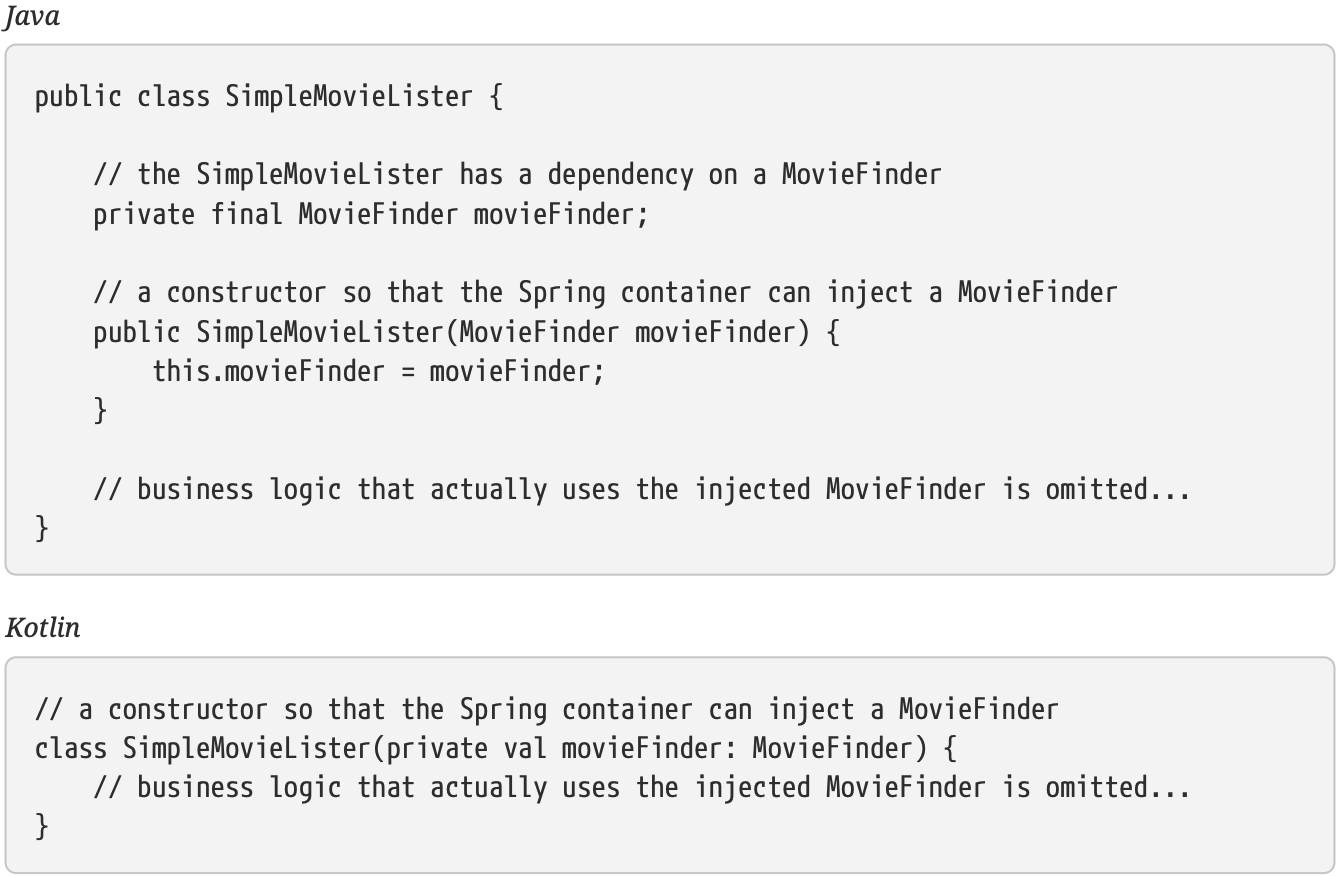
\includegraphics[width=1\linewidth]{./Figure/IMG_code_21.png}
\end{figure}

Notice that there is nothing special about this class. It is a POJO that has no dependencies on
container specific interfaces, base classes, or annotations.

\newpage
\textbf{Constructor Argument Resolution} Constructor argument resolution matching occurs by using the argument’s type. If no potential
ambiguity exists in the constructor arguments of a bean definition, the order in which the
constructor arguments are defined in a bean definition is the order in which those arguments are
supplied to the appropriate constructor when the bean is being instantiated. Consider the following
class:

\begin{figure}[ht]
    \centering
    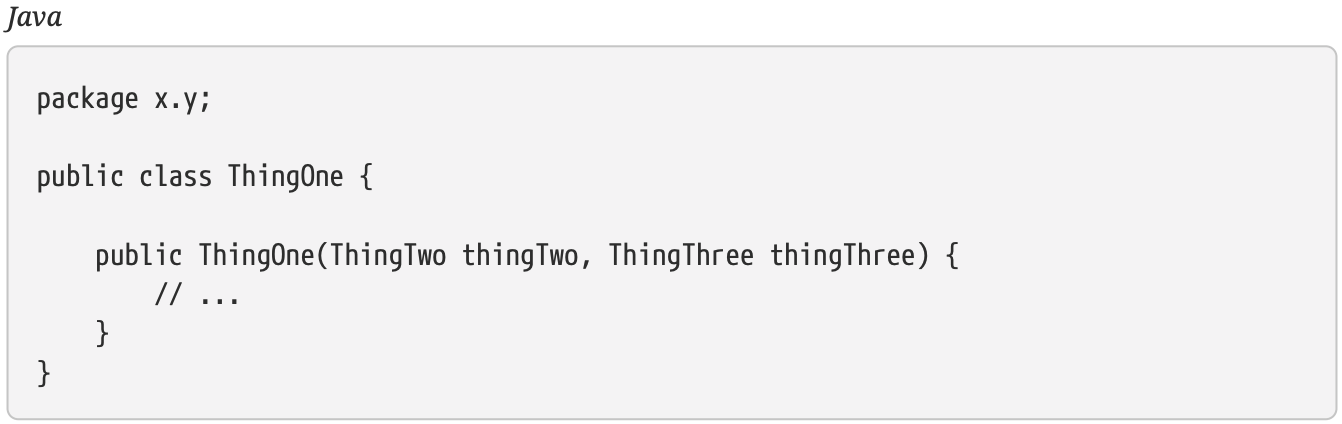
\includegraphics[width=1\linewidth]{./Figure/IMG_code_22.png}
\end{figure}
\begin{figure}[ht]
    \centering
    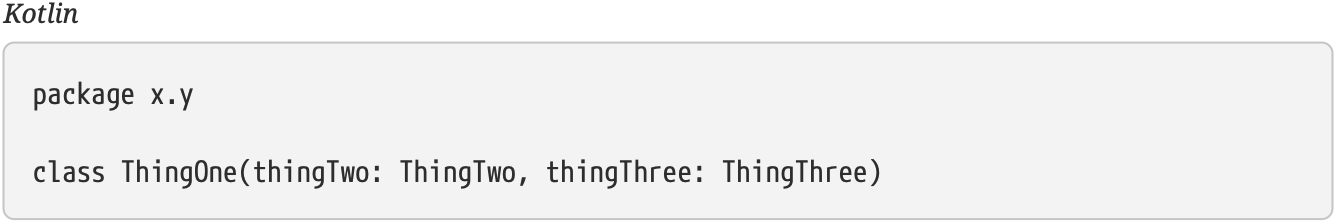
\includegraphics[width=1\linewidth]{./Figure/IMG_code_23.png}
\end{figure}

Assuming that the ThingTwo and ThingThree classes are not related by inheritance, no potential
ambiguity exists. Thus, the following configuration works fine, and you do not need to specify the
constructor argument indexes or types explicitly in the <constructor-arg/> element.

\begin{figure}[ht]
    \centering
    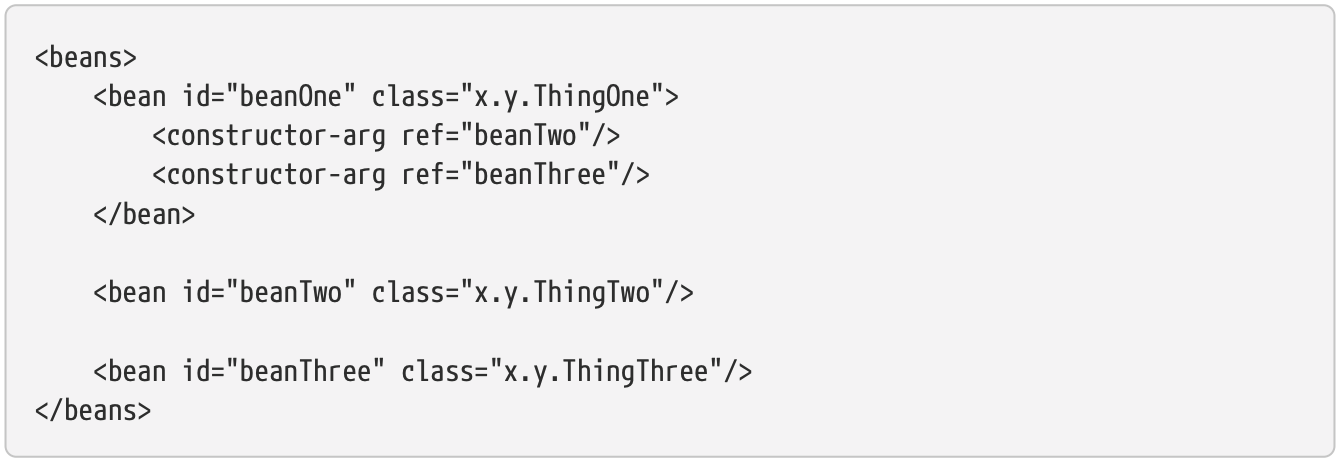
\includegraphics[width=1\linewidth]{./Figure/IMG_code_24.png}
\end{figure}

\newpage
When another bean is referenced, the type is known, and matching can occur (as was the case with
the preceding example). When a simple type is used, such as <value>true</value>, Spring cannot
determine the type of the value, and so cannot match by type without help. Consider the following
class:

\begin{figure}[ht]
    \centering
    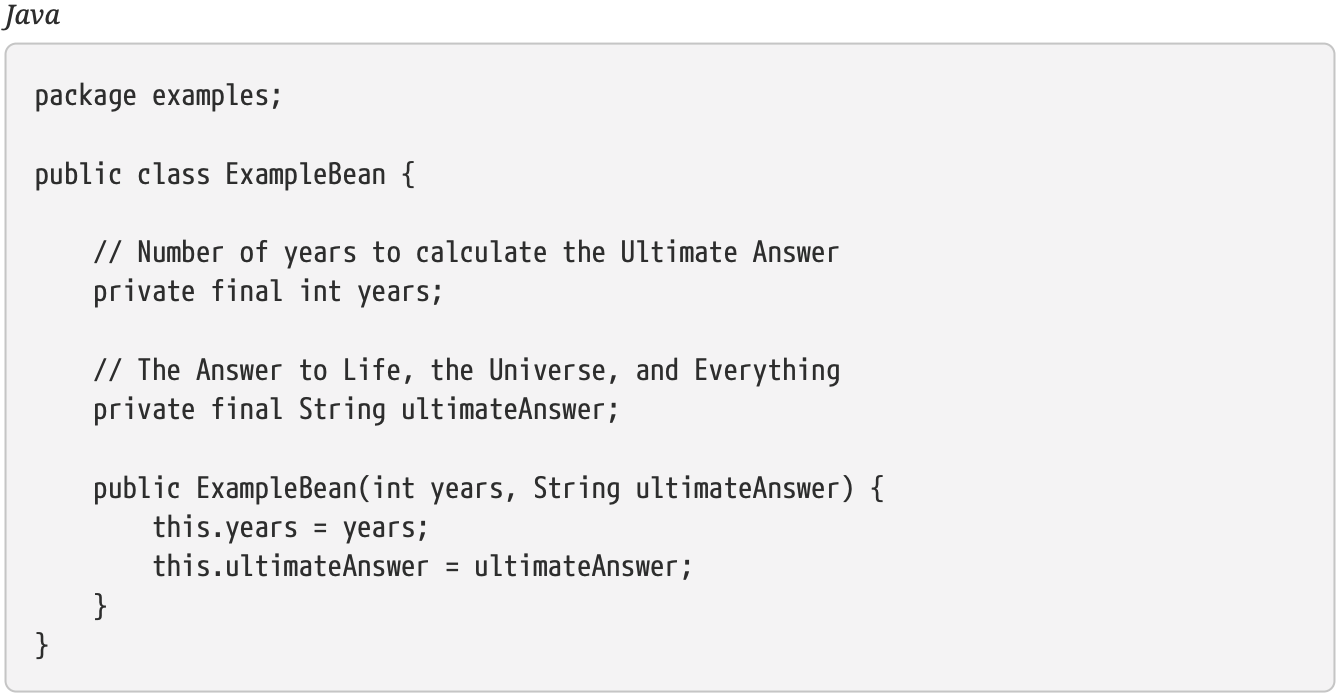
\includegraphics[width=1\linewidth]{./Figure/IMG_code_25.png}
\end{figure}

\begin{figure}[ht]
    \centering
    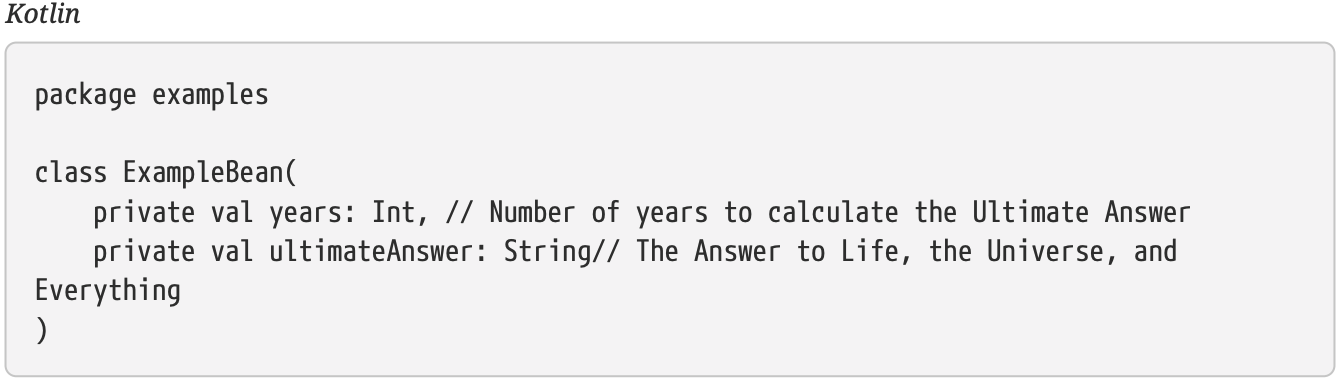
\includegraphics[width=1\linewidth]{./Figure/IMG_code_26.png}
\end{figure}

In the preceding scenario, the container can use type matching with simple types if you explicitly
specify the type of the constructor argument by using the type attribute, as the following example
shows:

\begin{figure}[ht]
    \centering
    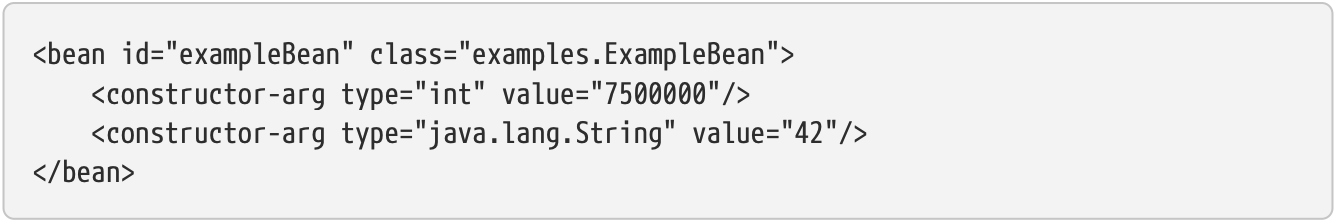
\includegraphics[width=1\linewidth]{./Figure/IMG_code_27.png}
\end{figure}
\newpage
You can use the index attribute to specify explicitly the index of constructor arguments, as the
following example shows:

\begin{figure}[ht]
    \centering
    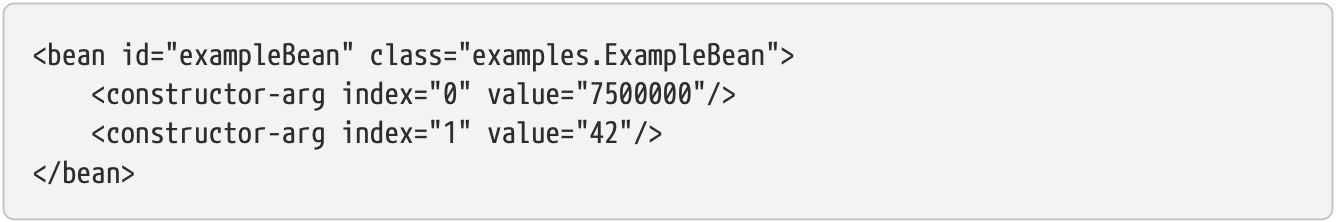
\includegraphics[width=1\linewidth]{./Figure/IMG_code_28.png}
\end{figure}

In addition to resolving the ambiguity of multiple simple values, specifying an index resolves
ambiguity where a constructor has two arguments of the same type.

You can also use the constructor parameter name for value disambiguation, as the following
example shows:

\begin{figure}[ht]
    \centering
    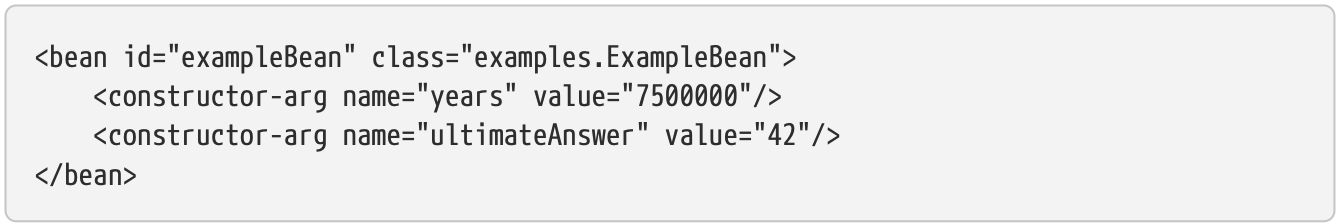
\includegraphics[width=1\linewidth]{./Figure/IMG_code_29.png}
\end{figure}

\newpage
Keep in mind that, to make this work out of the box, your code must be compiled with the debug
flag enabled so that Spring can look up the parameter name from the constructor. If you cannot or
do not want to compile your code with the debug flag, you can use the @ConstructorProperties JDK
annotation to explicitly name your constructor arguments. The sample class would then have to
look as follows:

\begin{figure}[ht]
    \centering
    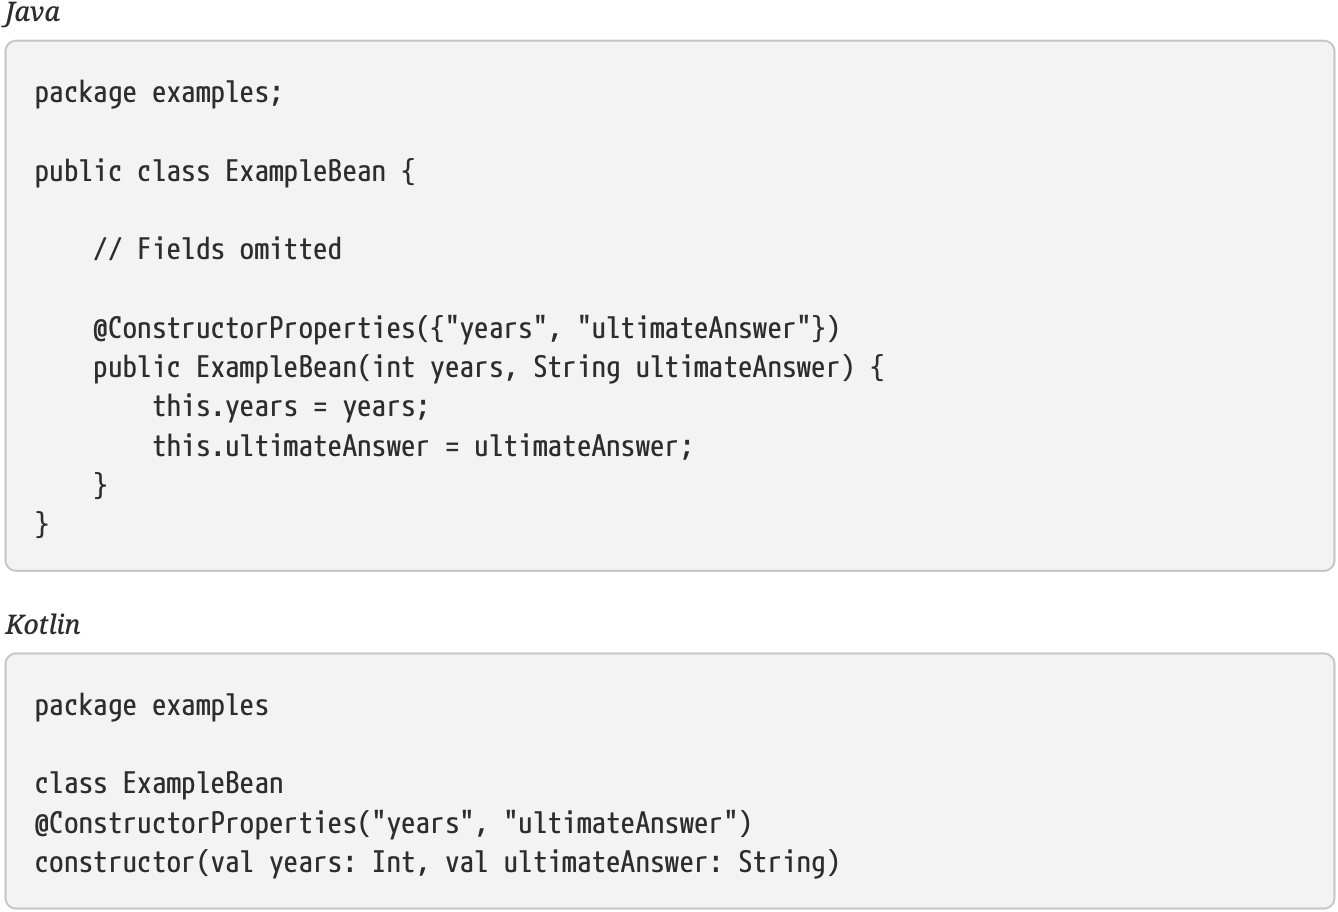
\includegraphics[width=1\linewidth]{./Figure/IMG_code_30.png}
\end{figure}

\subsubsection{Setter-based Dependency Injection}
Setter-based DI is accomplished by the container calling setter methods on your beans after
invoking a no-argument constructor or a no-argument static factory method to instantiate your
bean.

The following example shows a class that can only be dependency-injected by using pure setter
injection. This class is conventional Java. It is a POJO that has no dependencies on container specific
interfaces, base classes, or annotations.


\begin{figure}[ht]
    \centering
    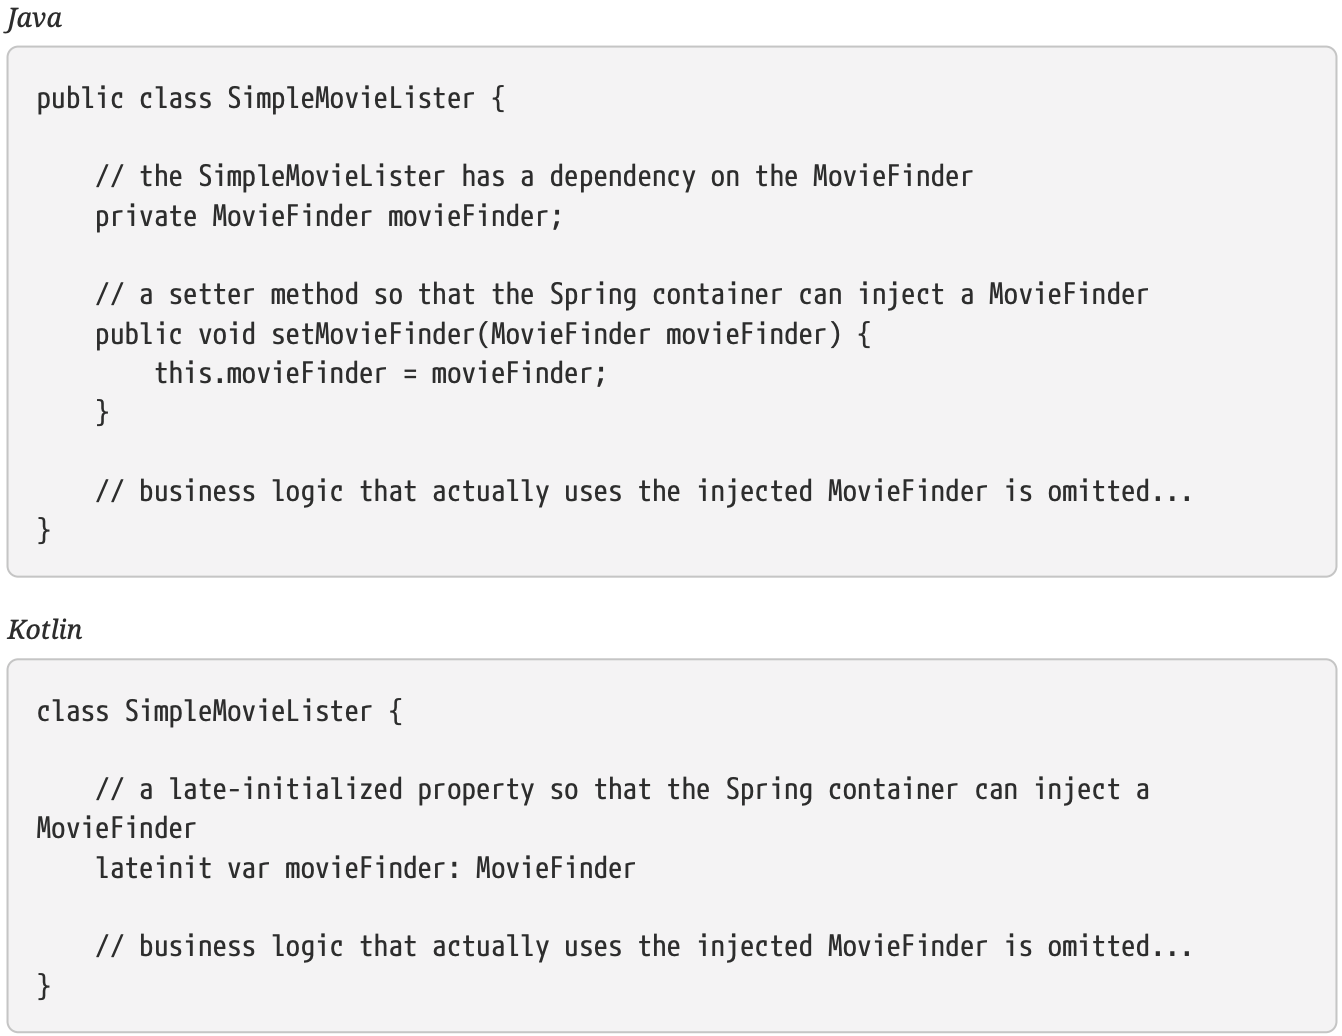
\includegraphics[width=1\linewidth]{./Figure/IMG_code_31.png}
\end{figure}


\chapter{Aspect Oriented Programming with Spring}
Aspect-oriented Programming (AOP) complements Object-oriented Programming (OOP) by
providing another way of thinking about program structure. The key unit of modularity in OOP is
the class, whereas in AOP the unit of modularity is the aspect. Aspects enable the modularization of
concerns (such as transaction management) that cut across multiple types and objects. (Such
concerns are often termed “crosscutting” concerns in AOP literature.)

One of the key components of Spring is the AOP framework. While the Spring IoC container does
not depend on AOP (meaning you do not need to use AOP if you don’t want to), AOP complements
Spring IoC to provide a very capable middleware solution.

AOP is used in the Spring Framework to:

\begin{itemize}
    \item Provide declarative enterprise services. The most important such service is declarative
    transaction management.
    \item Let users implement custom aspects, complementing their use of OOP with AOP.
\end{itemize}

\section{AOP Concepts}
Let us begin by defining some central AOP concepts and terminology. These terms are not Spring-specific. Unfortunately, AOP terminology is not particularly intuitive. However, it would be even
more confusing if Spring used its own terminology.

\begin{itemize}
    \item Aspect: A modularization of a concern that cuts across multiple classes. Transaction
    management is a good example of a crosscutting concern in enterprise Java applications. In
    Spring AOP, aspects are implemented by using regular classes (the schema-based approach) or
    regular classes annotated with the @Aspect annotation (the @AspectJ style).
    \item Join point: A point during the execution of a program, such as the execution of a method or the
    handling of an exception. In Spring AOP, a join point always represents a method execution.
    \item Advice: Action taken by an aspect at a particular join point. Different types of advice include
    “around”, “before” and “after” advice. (Advice types are discussed later.) Many AOP
    frameworks, including Spring, model an advice as an interceptor and maintain a chain of
    interceptors around the join point.
    \item Pointcut: A predicate that matches join points. Advice is associated with a pointcut expression
    and runs at any join point matched by the pointcut (for example, the execution of a method
    with a certain name). The concept of join points as matched by pointcut expressions is central to
    AOP, and Spring uses the AspectJ pointcut expression language by default.
    \item Introduction: Declaring additional methods or fields on behalf of a type. Spring AOP lets you
    introduce new interfaces (and a corresponding implementation) to any advised object. For
    example, you could use an introduction to make a bean implement an IsModified interface, to
    simplify caching. (An introduction is known as an inter-type declaration in the AspectJ
    community.)
    \item Target object: An object being advised by one or more aspects. Also referred to as the “advised
    object”. Since Spring AOP is implemented by using runtime proxies, this object is always a
    proxied object.
    \item AOP proxy: An object created by the AOP framework in order to implement the aspect contracts
    (advise method executions and so on). In the Spring Framework, an AOP proxy is a JDK dynamic
    proxy or a CGLIB proxy.
    \item Weaving: linking aspects with other application types or objects to create an advised object. This
    can be done at compile time (using the AspectJ compiler, for example), load time, or at runtime.
    Spring AOP, like other pure Java AOP frameworks, performs weaving at runtime.
\end{itemize}

Spring AOP includes the following types of advice:

\begin{itemize}
    \item Before advice: Advice that runs before a join point but that does not have the ability to prevent
    execution flow proceeding to the join point (unless it throws an exception).
    \item After returning advice: Advice to be run after a join point completes normally (for example, if a
    method returns without throwing an exception).
    \item After throwing advice: Advice to be run if a method exits by throwing an exception.
    \item After (finally) advice: Advice to be run regardless of the means by which a join point exits
    (normal or exceptional return).
    \item  Around advice: Advice that surrounds a join point such as a method invocation. This is the most
    powerful kind of advice. Around advice can perform custom behavior before and after the
    method invocation. It is also responsible for choosing whether to proceed to the join point or to
    shortcut the advised method execution by returning its own return value or throwing an
    exception.
\end{itemize}

Around advice is the most general kind of advice. Since Spring AOP, like AspectJ, provides a full
range of advice types, we recommend that you use the least powerful advice type that can
implement the required behavior. For example, if you need only to update a cache with the return
value of a method, you are better off implementing an after returning advice than an around
advice, although an around advice can accomplish the same thing. Using the most specific advice
type provides a simpler programming model with less potential for errors. For example, you do not
need to invoke the proceed() method on the JoinPoint used for around advice, and, hence, you
cannot fail to invoke it.

All advice parameters are statically typed so that you work with advice parameters of the
appropriate type (e.g. the type of the return value from a method execution) rather than Object
arrays.

The concept of join points matched by pointcuts is the key to AOP, which distinguishes it from older
technologies offering only interception. Pointcuts enable advice to be targeted independently of the
object-oriented hierarchy. For example, you can apply an around advice providing declarative
transaction management to a set of methods that span multiple objects (such as all business
operations in the service layer).

\section{Spring AOP Capabilities and Goals}
Spring AOP is implemented in pure Java. There is no need for a special compilation process. Spring
AOP does not need to control the class loader hierarchy and is thus suitable for use in a servlet
container or application server.

Spring AOP currently supports only method execution join points (advising the execution of
methods on Spring beans). Field interception is not implemented, although support for field
interception could be added without breaking the core Spring AOP APIs. If you need to advise field
access and update join points, consider a language such as AspectJ.

Spring AOP’s approach to AOP differs from that of most other AOP frameworks. The aim is not to
provide the most complete AOP implementation (although Spring AOP is quite capable). Rather, the
aim is to provide a close integration between AOP implementation and Spring IoC, to help solve
common problems in enterprise applications.

Thus, for example, the Spring Framework’s AOP functionality is normally used in conjunction with
the Spring IoC container. Aspects are configured by using normal bean definition syntax (although
this allows powerful “auto-proxying” capabilities). This is a crucial difference from other AOP
implementations. You cannot do some things easily or efficiently with Spring AOP, such as advise
very fine-grained objects (typically, domain objects). AspectJ is the best choice in such cases.
However, our experience is that Spring AOP provides an excellent solution to most problems in
enterprise Java applications that are amenable to AOP.

Spring AOP never strives to compete with AspectJ to provide a comprehensive AOP solution. We
believe that both proxy-based frameworks such as Spring AOP and full-blown frameworks such as
AspectJ are valuable and that they are complementary, rather than in competition. Spring
seamlessly integrates Spring AOP and IoC with AspectJ, to enable all uses of AOP within a consistent
Spring-based application architecture. This integration does not affect the Spring AOP API or the
AOP Alliance API. Spring AOP remains backward-compatible. See the following chapter for a
discussion of the Spring AOP APIs.

\section{AOP Proxies}
Spring AOP defaults to using standard JDK dynamic proxies for AOP proxies. This enables any
interface (or set of interfaces) to be proxied.

Spring AOP can also use CGLIB proxies. This is necessary to proxy classes rather than interfaces. By
default, CGLIB is used if a business object does not implement an interface. As it is good practice to
program to interfaces rather than classes, business classes normally implement one or more
business interfaces. It is possible to force the use of CGLIB, in those (hopefully rare) cases where
you need to advise a method that is not declared on an interface or where you need to pass a
proxied object to a method as a concrete type.

It is important to grasp the fact that Spring AOP is proxy-based. See Understanding AOP Proxies for
a thorough examination of exactly what this implementation detail actually means.